\documentclass[12pt]{article}
\usepackage{graphicx}
\usepackage{eso-pic}
\usepackage{ragged2e}
\usepackage{array}
\renewcommand\thepage{- \arabic{page} -}


\usepackage[utf8]{inputenc}
\usepackage[english]{babel}

\setlength{\parindent}{0em}
\setlength{\parskip}{1em}

%Logo
\newcommand\Highlight{%
	\put(0,150){%
		\parbox[b][\paperheight]{\paperwidth}{%
		\vfill
		\centering
		
\includegraphics[width=\paperwidth, height=10cm]{logo.jpg}%
		\vfill
}}}
%Swirl
\newcommand\Swirl{%
	\put(50,270){%
		\parbox[b][\paperheight]{\paperwidth}{%
		\vfill
		\centering
		
\includegraphics[width=20cm, height=20cm]{background.png}%
		\vfill
}}}
\graphicspath{{../images/}}
\usepackage{graphicx}


\AddToShipoutPicture*{\Highlight}
\AddToShipoutPictureBG{%
	\ifnum\value{page}>1
	\AtPageLowerLeft{\Swirl}%
    \fi
    }%

%Set default path for \input{…} akin to \graphicspath{…}
%https://tex.stackexchange.com/a/79060
\makeatletter
\providecommand*{\input@path}{}
\edef\input@path{{./FunctionalRequirements/}{./NonFunctionalRequirements/}{./OverallDescription/}{./PerformanceRequirements/}{./DesignConstraints/}{./Scope/}\input@path}% prepend
\makeatother


\begin{document}

{\fontfamily{phv}\selectfont % change phv to get new fonts for whole document
\font\myfont=cmr12 at 20pt

\begin{center}


\begin{minipage}{0.75\linewidth}


\vspace*{250pt}
\title{ \rule{\linewidth}{2pt} \\
\textbf{\normalfont\fontsize{35}{35}\scshape\selectfont IoT HomeCare System}\\
\textbf{\normalfont\fontsize{35}{35}\scshape\selectfont Architectural Design}\\}
\author{
        Hristian Vitrychenko\\
        Nikki Constancon \\
        Juan du Preez\\
        Gregory Austin \\
        Marthinus Richter
}
\date{\today \\ \rule{\linewidth}{2pt}}


\maketitle
\thispagestyle{empty}

\end{minipage}
\end{center}
\pagebreak

\clearpage

\section{Introduction}
\subsection{Purpose}
The purpose of this document is to provide a detailed representation of the ReVA system. This document clearly illustrates and explains the chosen architectural designs of the different parts of the whole system. The system is shown to have different subsystems, and several specific artifacts in the system are explained with the use of diagrams and short summaries in order to make clear how the system is meant to work.
\subsection{Definitions}
\subsection{References}
\subsection{Overview}
The document begins by giving an overall description of the system in the form of a deployment diagram. After that, the separate subsystems are shown and explained in terms of system types and appropriate architectural designs chosen for them. Then, each artifact within the deployment diagram is given its own class diagram and/or other diagrams which clearly expresses the designs and reasons for the chosen designs.

\clearpage
\section{Overall Description}
\subsection{Deployment Diagram}
\begin{center}
\begin{figure}[h]
	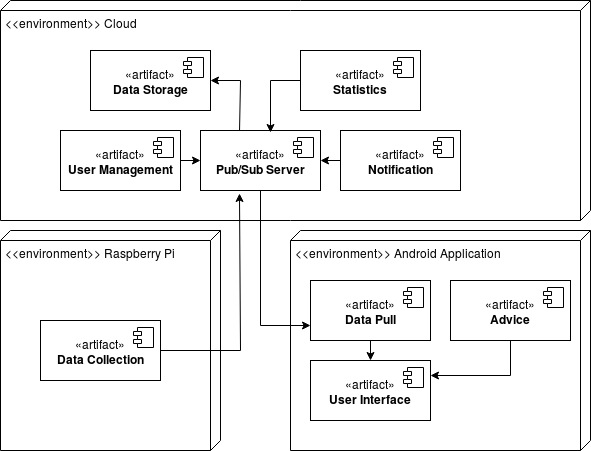
\includegraphics[width=15cm, height=10cm]{OverallDescription/DeploymentDiagram.png}
\end{figure}
\end{center}

\subsection{System and Subsystems}
	The ReVA (Revolutionary Vitality Analyzer) system is the overall system and does not necessarily have a system type, as it is composed of many different subsystems which have their own types and perform different functions as specified in the SRS. If one looks at the system as a whole, it would be an interactive system. This implies that the Android App speaks with and interacts with the server in order to get data from the Raspberry Pi. This is implemented in the Client-Server design. The following subsystems comprise the entire system.

\begin{itemize}
	\item \textbf{Real-Time Subsystem}\\
	This subsystem is responsible for collecting the data, and displaying it real-time on the mobile application. The artifacts which are used are: Data Collection,  Pub/Sub Server, Data Pull, and User Interface. The type of system is a blackboard system since the Data Collection artifact will publish data constantly on the "blackboard" Pub/Sub Server which is situated on the cloud itself. This system is most appropriate because of the constant stream of data, which can be used by subscribers such as the Android application and other modules or artifacts. 
	\item \textbf{Data Storage Subsystem}\\
	This system is responsible for the CRUD functionality of data. It is therefore a persistence framework, and hence a persistence architectural design. The Data Storage artifact subscribes to the Pub/Sub Server, or connects to it by other means, and fills the Cassandra database with data in a format that is ready for research analysis. The persistence is chosen because it fits well with the need for researchers to analyse data, as well as providing an interface for the Statistics module. 
	\item \textbf{History/Statistics Subsystem}\\
	The Data Storage, Statistics, Pub/Sub Server, and User Interface modules work together to provide the user with History and or Statistical data in the form of points on a graph ready to be plotted. This would be an interactive system with a client-server design. The user makes requests via the User Interface to the server which in turn makes use of the Statistics module. The Statistics module gets data from the Data Storage module, and generates the response which the server will return to the user.
	\item \textbf{User Management Subsystem}\\
	All the management of user accounts and sessions, such as registration and logging in/ out, will be handled by the User Management. This is a combination of a client-server and a persistence architecture. Registration etc. requests are originated by the user via the User Interface. This issues a request to the server which consults the User Management module to update a database. 
	\item \textbf{Notification Subsystem}\\
	The notification subsystem is an event-driven type of system. The Notification module is subscribed to the Pub/Sub server, and receives data all the time, analysing it for possible issues. It only reacts to certain events, i.e. in the event of an emergency. This is appropriate because it is completely state-dependent. Reactions and particular alerts are dependent on the states of the data, whether they fall within certain criteria or not.
	\item \textbf{Advice Subsystem}\\
	This subsystem is somewhat of a persistence framework. It is static advice on the app itself, such that the user can know what to do in emergencies. The only modules used are Advice and User Interface.
\end{itemize}

\clearpage
\section{Detailed Artifact Descriptions}
	\subsection{Raspberry Pi Environment}
		\subsubsection{Data Collection}
		%diagram
%description
%design patterns
	\subsection{Cloud Server Environment}
		\subsubsection{Pub/Sub Server}
		\subsubsection{Data Storage}
		\subsubsection{Statistics}
		\subsubsection{Notification}
		\subsubsection{User Management}
	\subsection{Android Application Environment}	
		\subsubsection{User Interface}
		\subsubsection{Data Pull}
		\subsubsection{Advice}
		
\clearpage
\section{Conclusion}
%\input{introduction/design_constraints}
  
\end{document}
